\section{Results}

The results below describe the current COMSOL model-development status. They should be interpreted as controlled internal comparisons rather than validation against measured Early Warning Scan data. Unless stated otherwise, the current Tier 1 values are extracted from existing COMSOL outputs at the case-specific review time.

\subsection{Pipeline status}

The COMSOL pipeline can generate model variants from TOML files, expand source-case settings, construct COMSOL Java builder scripts, run build-only checks, run transient studies where appropriate, and export summary metrics and plots. The pipeline has also been reorganized so that normal COMSOL runs no longer import the older FEBio-oriented package. The active source-case settings, lobule generation, TOML I/O, and optional mesh-generation support now live inside \texttt{ews\_fem\_pipeline\_comsol}.

The current clean evaluation output is stored under \texttt{analysis\_output/comsol\_pipeline}. The most important current comparison folders are \texttt{tier1\_comparison} and \texttt{tier1\_comparison\_without\_stage1}. The latter is useful because Stage 1 has a different simple geometry and larger volume than the later anatomical route.

\begin{table}[H]
\centering
\small
\caption{Current report-ready status of the main COMSOL branches.}
\label{tab:completed_branches}
\begin{tabular}{p{0.18\linewidth} p{0.28\linewidth} p{0.39\linewidth}}
\toprule
Branch & Completed outputs & Report interpretation \\
\midrule
Stage 1 motion baseline & Complete 0.25g dynamic output & Motion sanity baseline only; not a fair anatomical comparator. \\
Stage 2 chestwall & Complete xoffset055 output & First fair anatomical baseline for later stages. \\
Stage 3 realistic glandular & Complete realistic reference output & Main current anatomical glandular reference. \\
Stage 4 reference & Complete no-asymmetry control & Control case for later asymmetry sensitivities. \\
Stage 5 no-Cooper & Complete no-Cooper control & Control case; stable Cooper effect not proven yet. \\
Stage 6 tumor & Build-only and screening cases prepared & Tumor-mask sensitivity route; quantitative results only after valid solves. \\
\bottomrule
\end{tabular}
\end{table}

\subsection{Tier 1 comparison}

Table~\ref{tab:tier1_results} summarizes the current Tier 1 comparison. Stage 1 has a substantially larger volume and simpler geometry, so its displacement and stress values should not be interpreted as an anatomical baseline for Stages 2--5. Stage 2 is the first fair anatomical baseline. Stages 3, 4, and 5 are intentionally similar because Stage 4 is a no-asymmetry control and Stage 5 is a no-Cooper control.

\begin{table}[H]
\centering
\small
\caption{Current Tier 1 COMSOL comparison. VM denotes von Mises stress.}
\label{tab:tier1_results}
\begin{tabular}{lrrrrr}
\toprule
Case & Breast & Gland & Avg disp. & Mean VM & Max VM \\
 & (mL) & (\%) & (mm) & (kPa) & (kPa) \\
\midrule
Stage 1 0.25g baseline & 718.72 & 11.94 & 17.76 & 0.433 & 10.73 \\
Stage 2 xoffset055 chestwall & 585.06 & 9.16 & 3.03 & 0.311 & 1.35 \\
Stage 3 realistic glandular & 585.09 & 24.31 & 3.00 & 0.324 & 1.67 \\
Stage 4 realistic reference & 585.09 & 24.31 & 3.00 & 0.324 & 1.63 \\
Stage 5 no-Cooper control & 585.09 & 24.31 & 3.00 & 0.324 & 1.61 \\
\bottomrule
\end{tabular}
\end{table}

The large difference between Stage 1 and Stage 2 is expected. Stage 1 used a simple baseline geometry with a breast volume of approximately 719 mL, while Stage 2 introduced the selected xoffset055 chestwall route with a volume of approximately 585 mL. The reduction in average displacement from 17.76 mm to about 3.03 mm therefore reflects both geometry and volume changes, not only the chestwall curvature.

The small differences between Stages 3--5 are also expected. Stage 3 adds the realistic glandular reference. Stage 4 keeps this reference but disables asymmetry, and Stage 5 keeps the same reference while disabling Cooper support. These cases are controls, not three independent active sensitivities.

\subsection{Stage 1: dynamic motion sanity baseline}

Stage 1 validates the mild fixed-support acceleration pulse. The pulse amplitude is 0.25g and the duration is 0.60 s. The case reached the expected end time of 2.2 s and produced complete metrics. Because its geometry and volume differ from the selected anatomical route, it is reported as a motion baseline rather than as the final anatomical reference.

\begin{figure}[H]
\centering
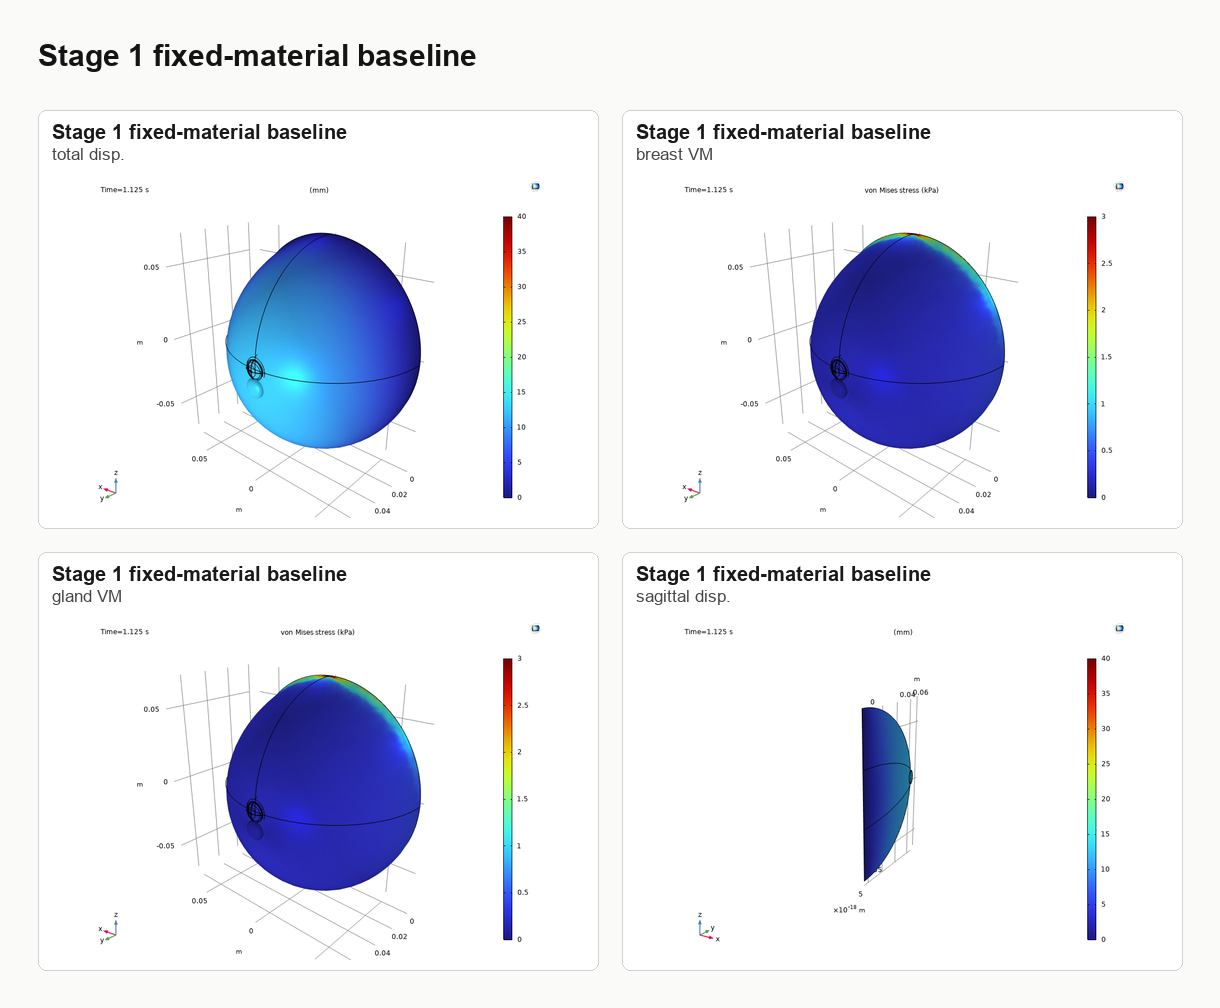
\includegraphics[width=0.95\linewidth,height=0.78\textheight,keepaspectratio]{Figures/comsol_contact_sheets/stage1_baseline_contact_sheet.png}
\caption{Stage 1 baseline contact sheet. This case is used to validate the dynamic 0.25g motion input and should not be interpreted as the final anatomical baseline.}
\label{fig:stage1_contact_sheet}
\end{figure}

\subsection{Stage 2: selected chestwall geometry}

Stage 2 introduces the selected transverse chestwall curvature with approximately +55 mm x-offset, volume-preserving compensation, and automatic nipple/gland alignment. This is the first fair anatomical baseline for later stages. The current case reached the expected end time of 2.2 s and produced a breast volume of 585.06 mL, glandular fraction of 9.16\%, average review displacement of 3.03 mm, mean breast VM stress of 0.311 kPa, and maximum breast VM stress of 1.35 kPa.

\begin{figure}[H]
\centering
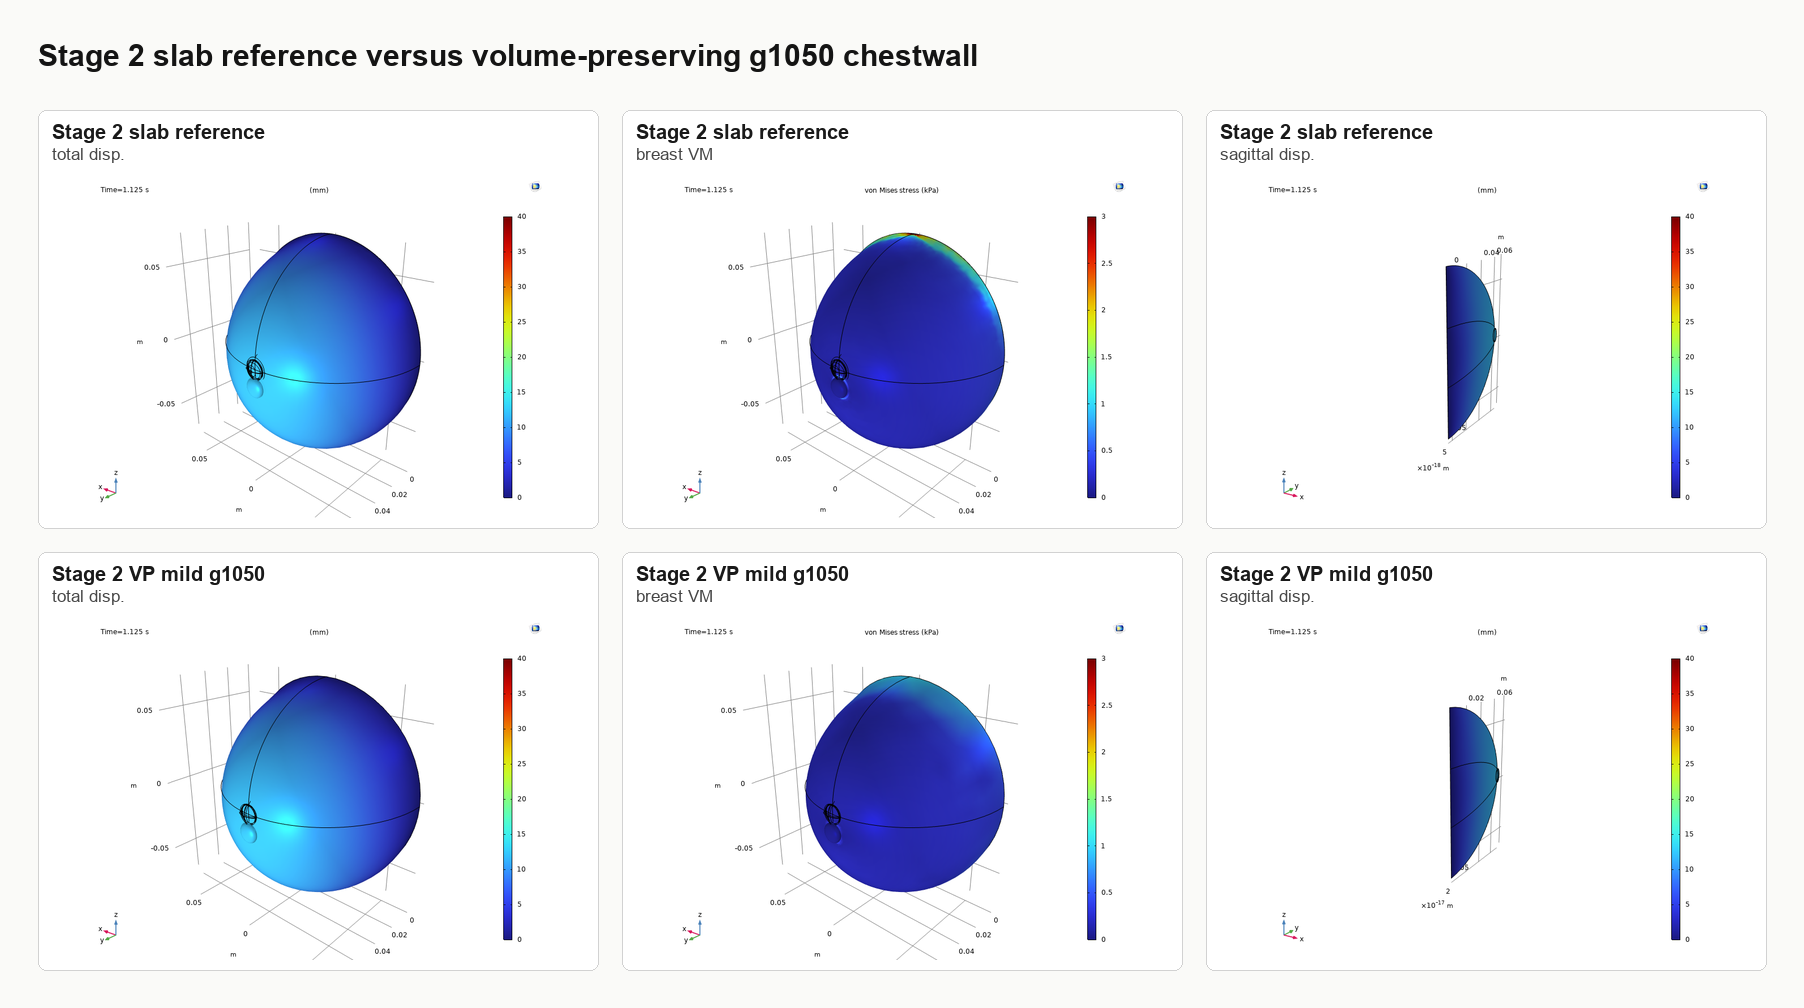
\includegraphics[width=0.95\linewidth,height=0.78\textheight,keepaspectratio]{Figures/comsol_contact_sheets/stage2_chestwall_contact_sheet.png}
\caption{Stage 2 contact sheet for the selected chestwall route. The xoffset055 case is the first fair anatomical baseline for later model stages.}
\label{fig:stage2_contact_sheet}
\end{figure}

\subsection{Stage 3: realistic glandular reference}

Stage 3 adds the realistic chestwall-aware glandular lobule spread to the selected Stage 2 chestwall geometry. This raises the glandular fraction from about 9.16\% to about 24.31\% while preserving the breast volume near 585 mL. The current Tier 1 output reached 2.2 s and produced an average review displacement of 3.00 mm, mean breast VM stress of 0.324 kPa, and maximum breast VM stress of 1.67 kPa.

The result suggests that the realistic glandular reference can be added without causing a large global change in the current mild dynamic response. This is not a negative result: it means that the current Stage 3 reference is a controlled anatomical refinement rather than an aggressive mechanical perturbation. Additional compact/reference/wide spread variants are still needed to isolate the effect of glandular spatial distribution at matched glandular volume.

\begin{figure}[H]
\centering
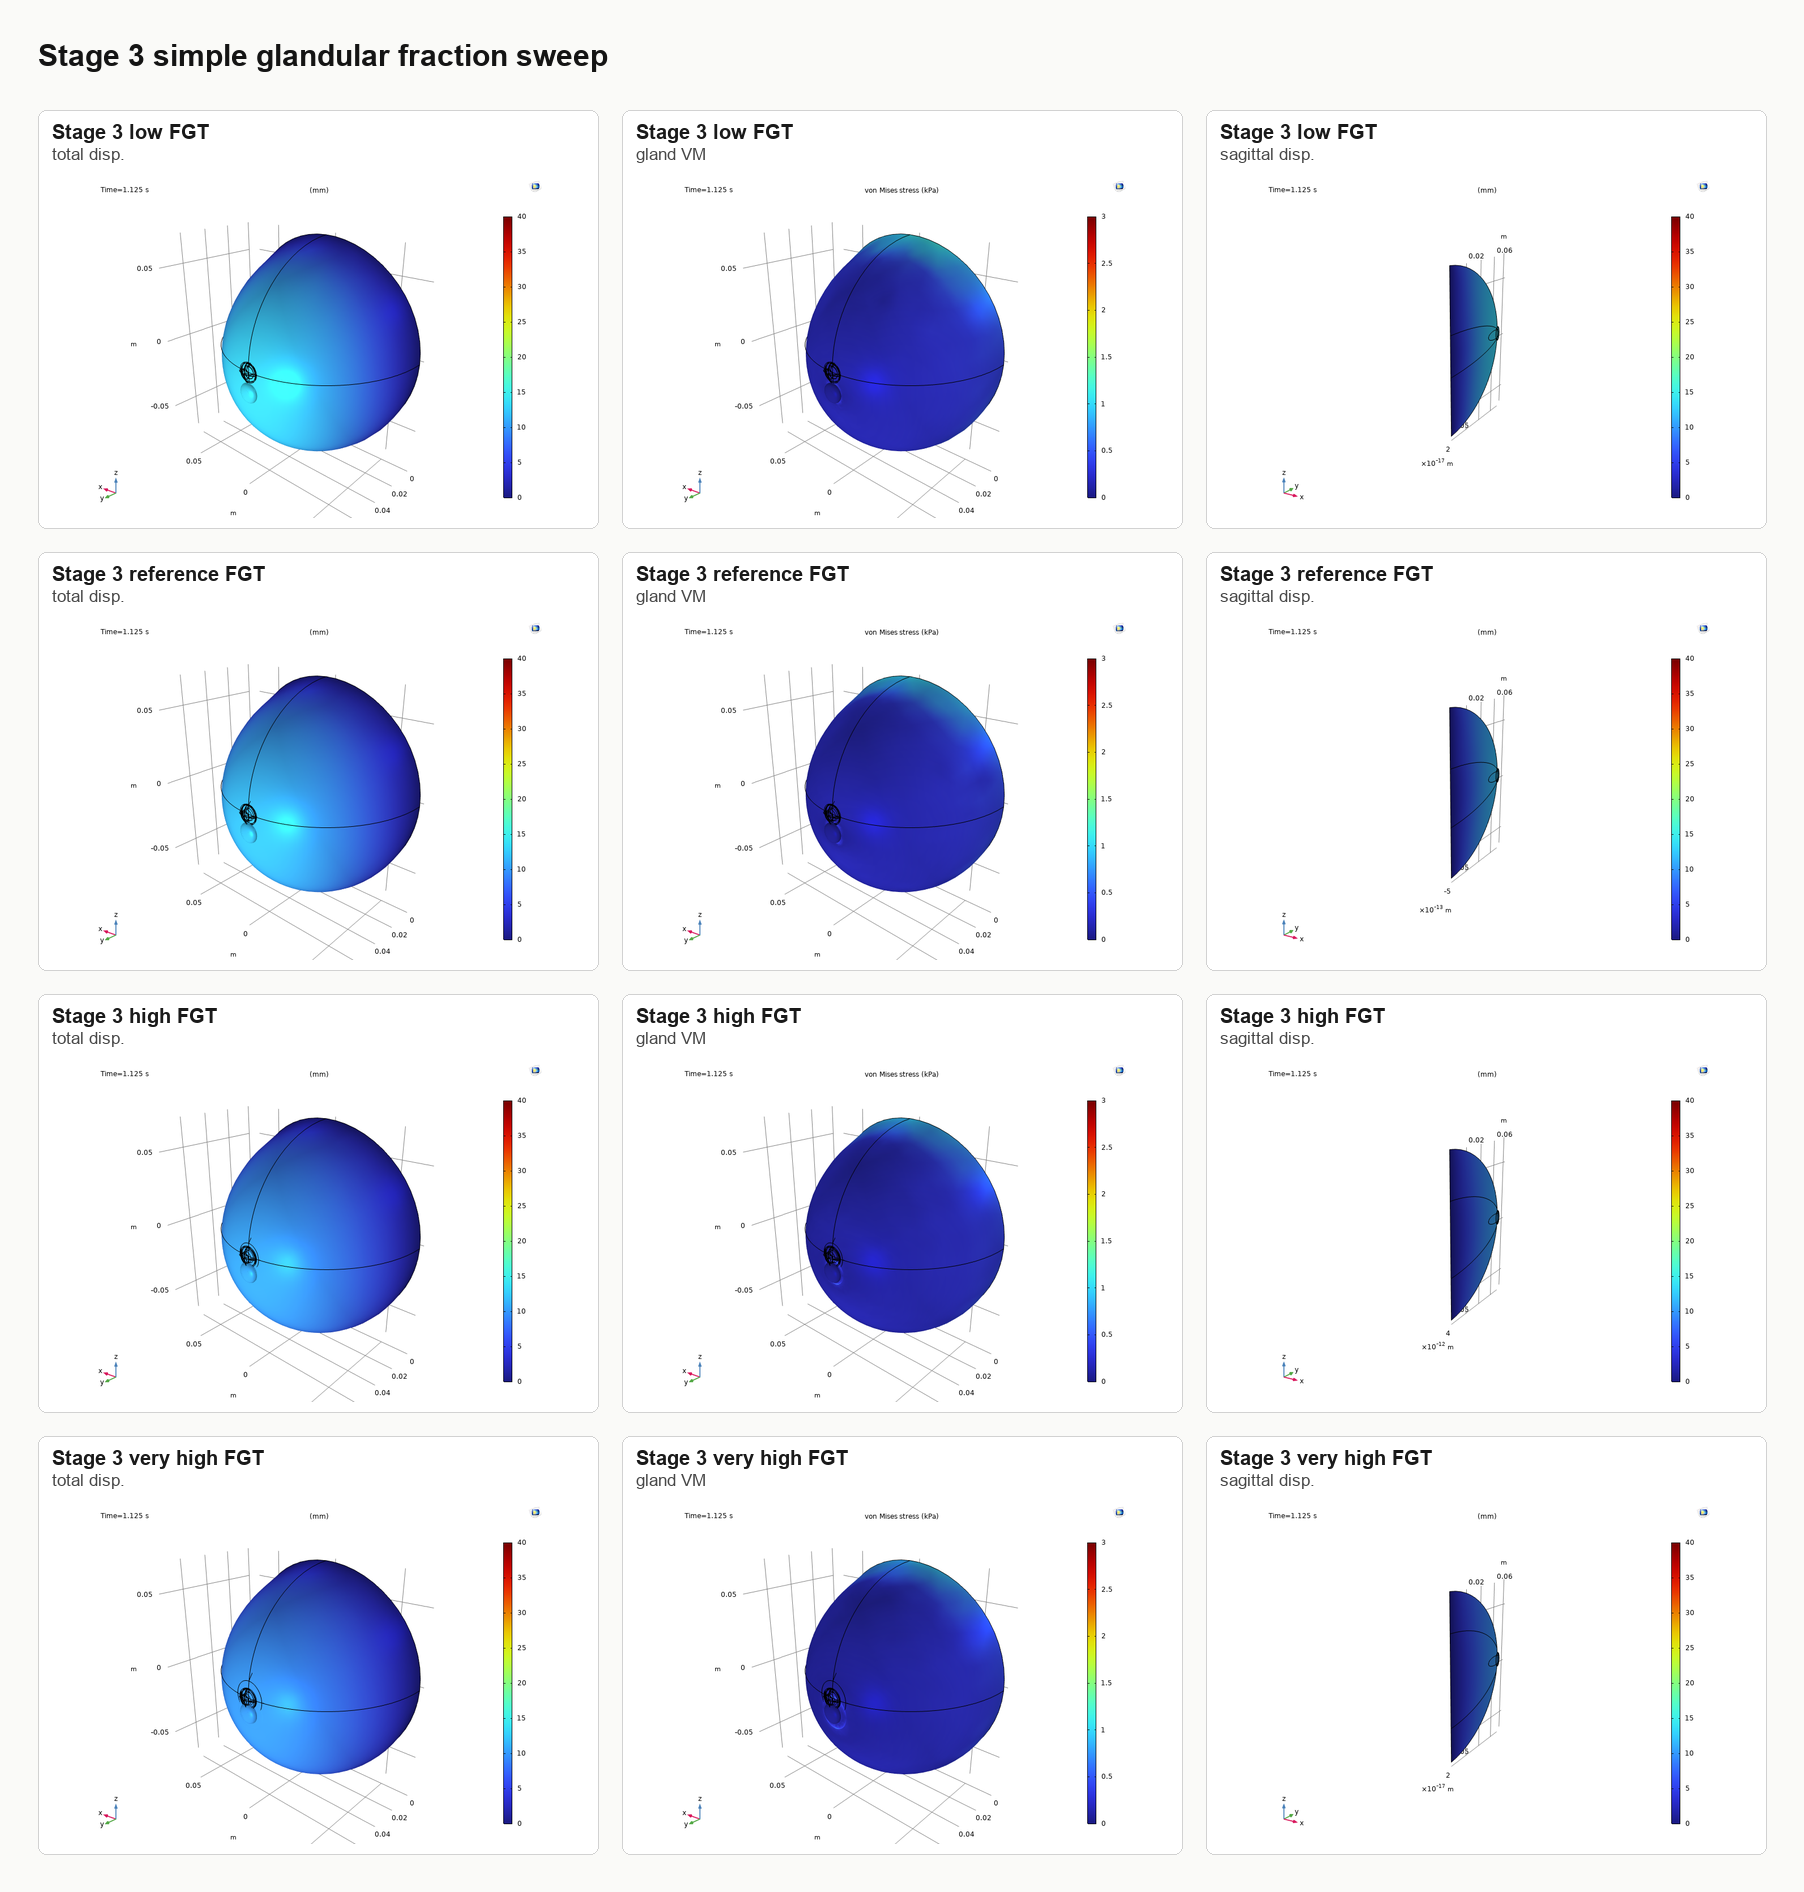
\includegraphics[width=0.95\linewidth,height=0.78\textheight,keepaspectratio]{Figures/comsol_contact_sheets/stage3_glandular_fraction_contact_sheet.png}
\caption{Stage 3 contact sheet. The current report interpretation separates the solved simple fraction sweep from the newer realistic glandular reference, which is used in the Tier 1 anatomical route.}
\label{fig:stage3_contact_sheet}
\end{figure}

\subsection{Stage 4: asymmetry control}

The current Tier 1 Stage 4 entry is a realistic reference/control case with profile asymmetry disabled. It is intentionally almost identical to the Stage 3 realistic reference. Its purpose is to provide a clean reference for later asymmetry tests, not to prove an asymmetry effect by itself. The output reached 2.2 s and produced nearly the same values as Stage 3: 585.09 mL breast volume, 24.31\% glandular fraction, 3.00 mm average review displacement, and 0.324 kPa mean breast VM stress.

Earlier additive lateral or fullness ellipsoid asymmetry cases should not be used as report evidence, because they could create misleading extra volumes in the final breast union. The preferred future asymmetry route is surface/profile deformation with nipple and glandular alignment.

\begin{figure}[H]
\centering
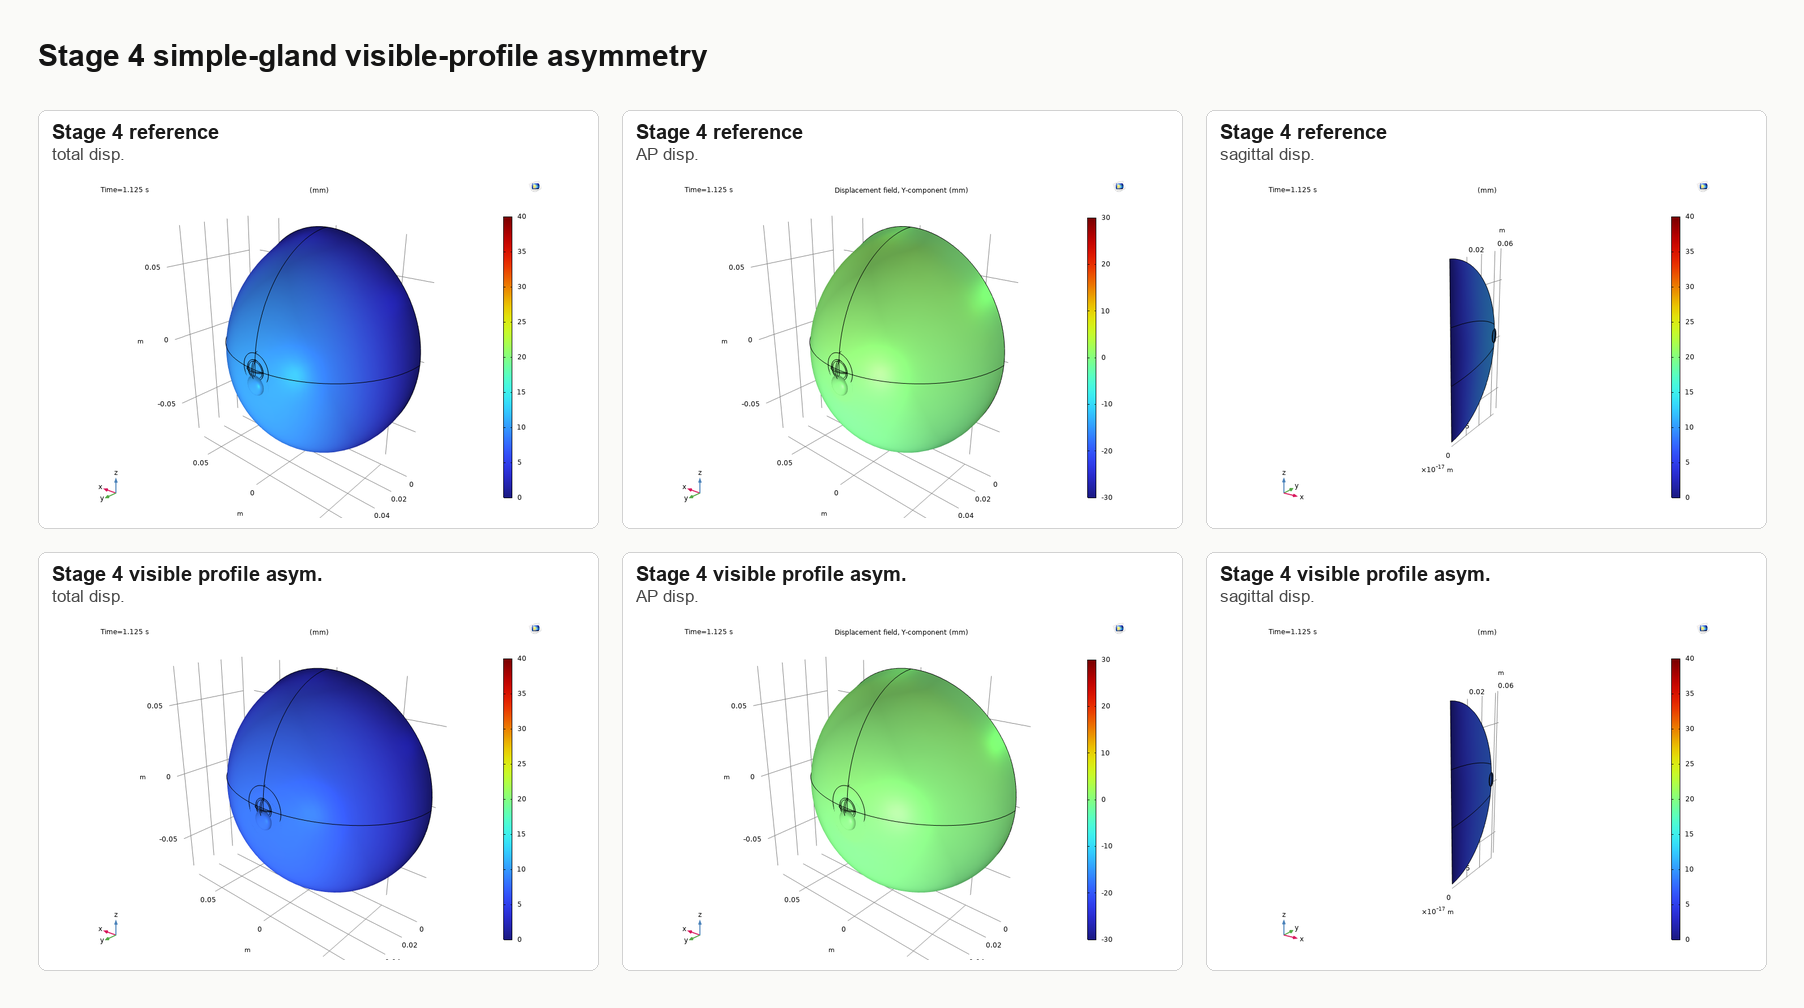
\includegraphics[width=0.95\linewidth,height=0.78\textheight,keepaspectratio]{Figures/comsol_contact_sheets/stage4_asymmetry_contact_sheet.png}
\caption{Stage 4 contact sheet. Stage 4 should currently be interpreted as a control and sensitivity framework rather than as a completed patient-specific asymmetry model.}
\label{fig:stage4_contact_sheet}
\end{figure}

\subsection{Stage 5: no-Cooper control}

Stage 5 currently provides a matched no-Cooper control on top of the Stage 3/4 realistic reference geometry. This case reached 2.2 s and produced values almost identical to Stage 3 and Stage 4. This is expected because the Cooper scaffold is disabled in the Tier 1 Stage 5 entry.

The default Stage 5B Cooper run is not report-ready because it failed almost immediately around $t = 2.148 \times 10^{-6}$ s with nonlinear solver/out-of-core problems. Therefore, the current Tier 1 comparison does not demonstrate a reliable Cooper-ligament support effect. Cooper ligament modelling should be reported as a mechanical support sensitivity that still requires a stable mild variant.

\begin{figure}[H]
\centering
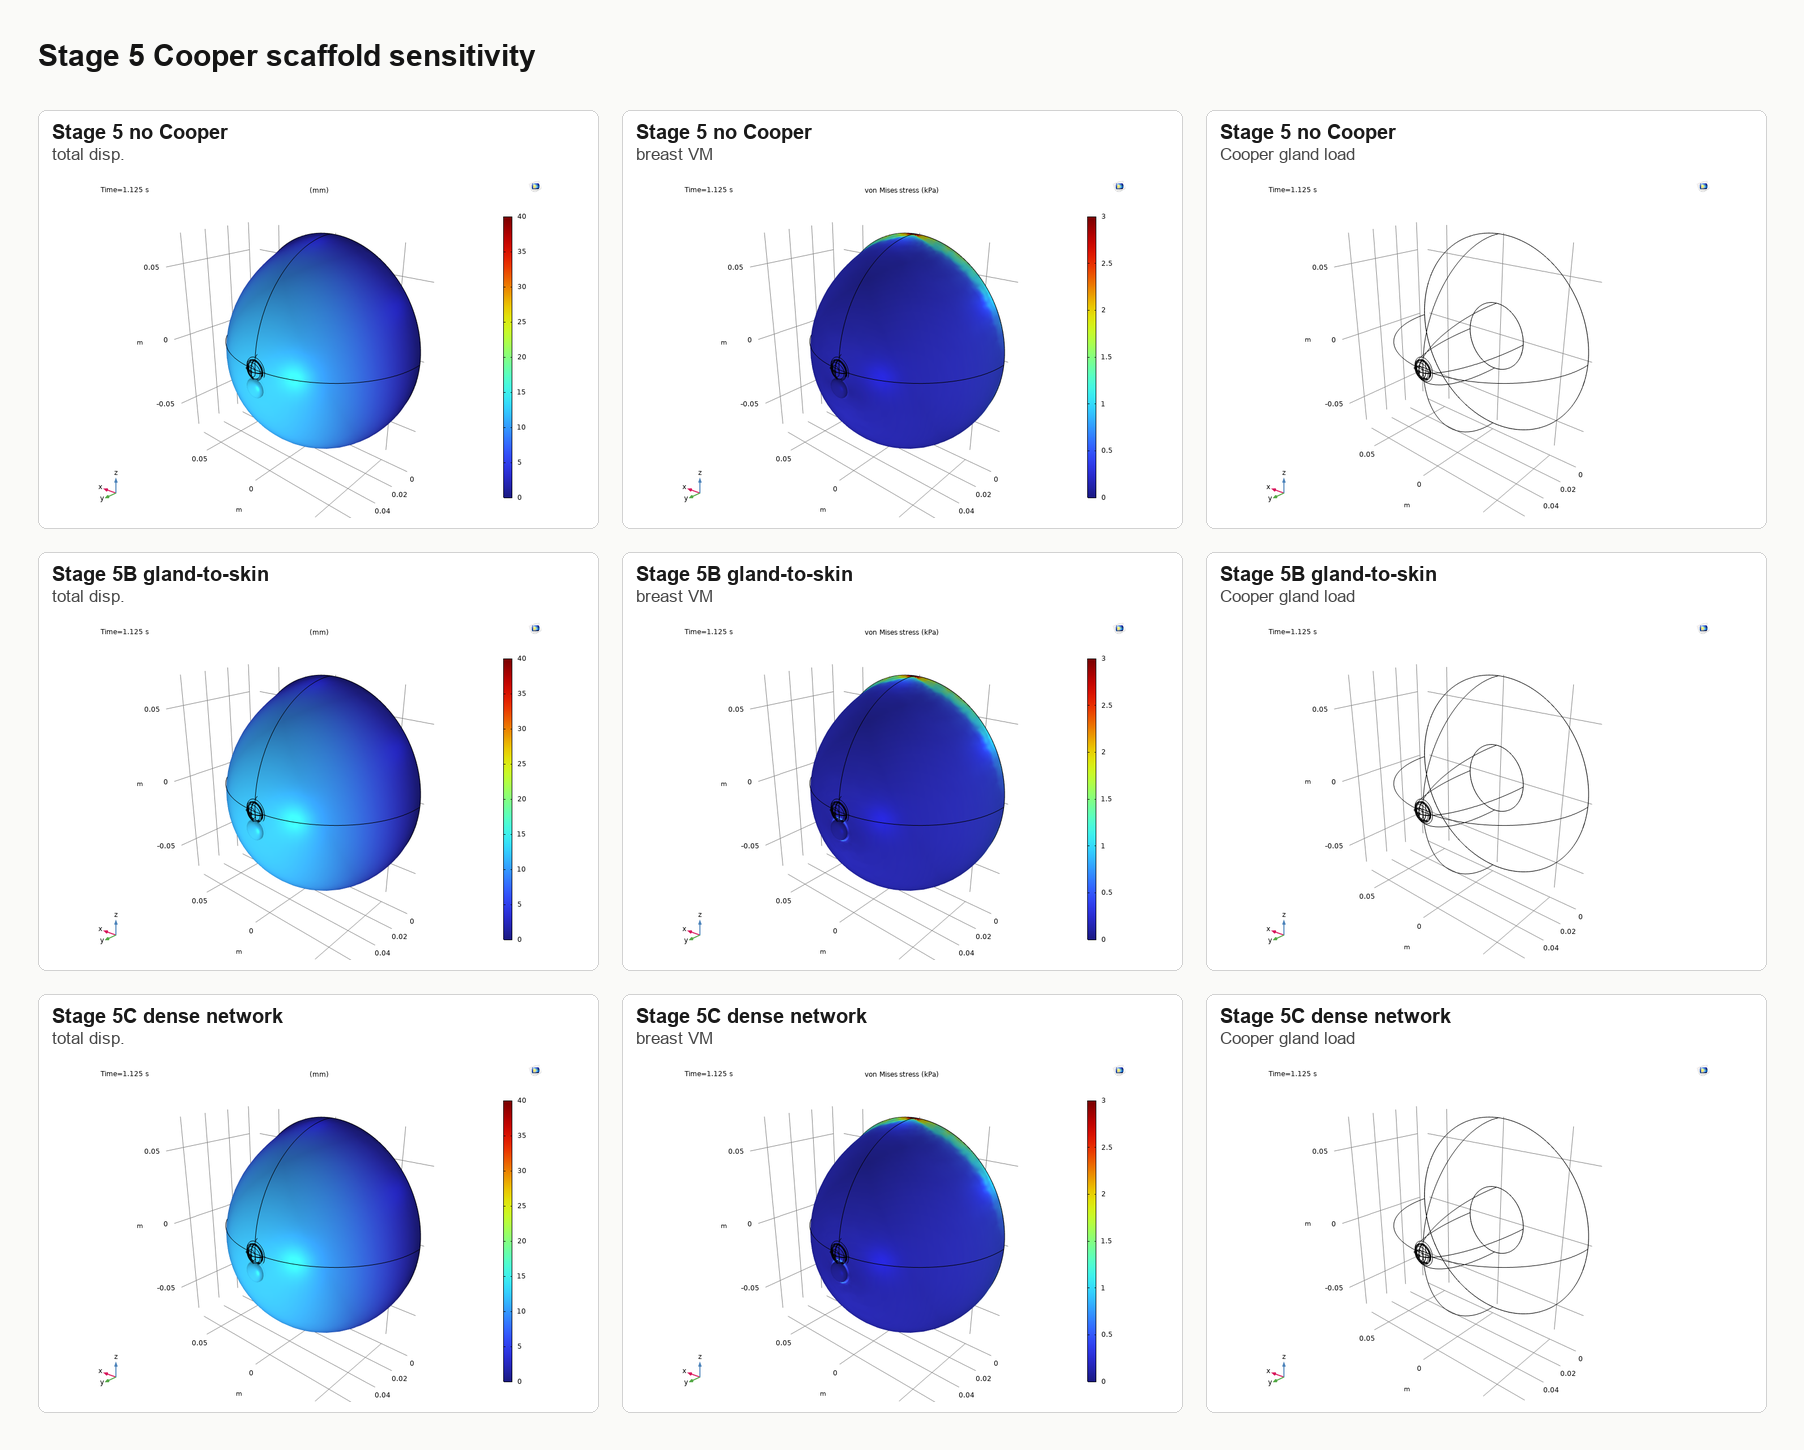
\includegraphics[width=0.95\linewidth,height=0.78\textheight,keepaspectratio]{Figures/comsol_contact_sheets/stage5_cooper_contact_sheet.png}
\caption{Stage 5 contact sheet. The current robust case is the no-Cooper control; Cooper support remains a sensitivity route requiring a stable solved variant.}
\label{fig:stage5_contact_sheet}
\end{figure}

\subsection{Stage 5: skin-layer and material scout}

After the no-Cooper control was established, a diagnostic skin-layer scout was performed to test whether a separate volumetric skin layer could be added without the nonphysical deformation observed in the earlier shell-scaffold skin route. The shell/scaffold route produced visible dimples and surface artefacts during motion and is therefore not used as a main result. The volumetric skin case produced a visually stable motion pattern, but it substantially reduced the displacement amplitude.

Table~\ref{tab:stage5_skin_scout} summarizes the manual Derived Values comparison. All four cases use the matched Stage 5 no-Cooper anatomy and the same breast volume of approximately 585 mL. The comparison should be interpreted as a scout because the values were exported manually from COMSOL tables and do not include the full automated surface or landmark post-processing.

\begin{table}[H]
\centering
\small
\caption{Manual Stage 5 skin/material scout. VM denotes von Mises stress.}
\label{tab:stage5_skin_scout}
\begin{tabular}{lrrrr}
\toprule
Case & Peak avg disp. & Peak max disp. & Peak avg VM & Peak max VM \\
 & (mm) & (mm) & (kPa) & (kPa) \\
\midrule
No skin, 1.00g & 6.48 & 12.51 & 0.709 & 3.47 \\
No skin, 1.25g & 7.34 & 14.23 & 0.805 & 3.92 \\
Volumetric skin, 1.25g & 3.40 & 5.93 & 1.379 & 51.63 \\
Vol. skin + soft interior, 1.25g & 5.90 & 10.90 & 1.801 & 72.38 \\
\bottomrule
\end{tabular}
\end{table}

Increasing the acceleration from 1.00g to 1.25g in the no-skin model increased peak maximum displacement from 12.51 mm to 14.23 mm. In contrast, adding the volumetric skin layer at 1.25g reduced the peak maximum displacement to 5.93 mm. Softening the adipose and glandular interior while retaining the volumetric skin increased the peak maximum displacement to 10.90 mm. This indicates that the current volumetric skin implementation has a larger effect on the global motion amplitude than the 1.00g to 1.25g excitation change, and that internal tissue compliance partly compensates for this damping.

\begin{figure}[H]
\centering
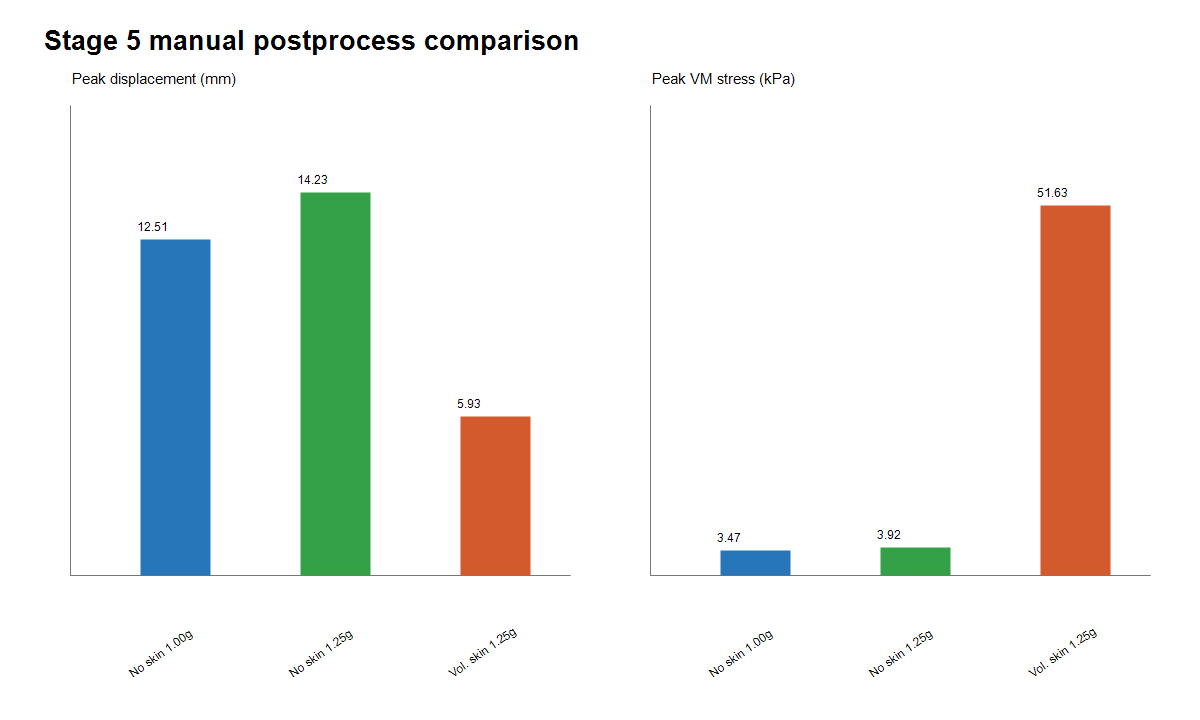
\includegraphics[width=0.95\linewidth]{Figures/stage5_manual_postprocess/stage5_manual_peak_comparison.png}
\caption{Manual Stage 5 peak comparison from COMSOL Derived Values. The volumetric skin case strongly damps displacement, while the soft-interior variant partially recovers displacement at the cost of higher localized maximum VM stress.}
\label{fig:stage5_skin_scout_peaks}
\end{figure}

\begin{figure}[H]
\centering
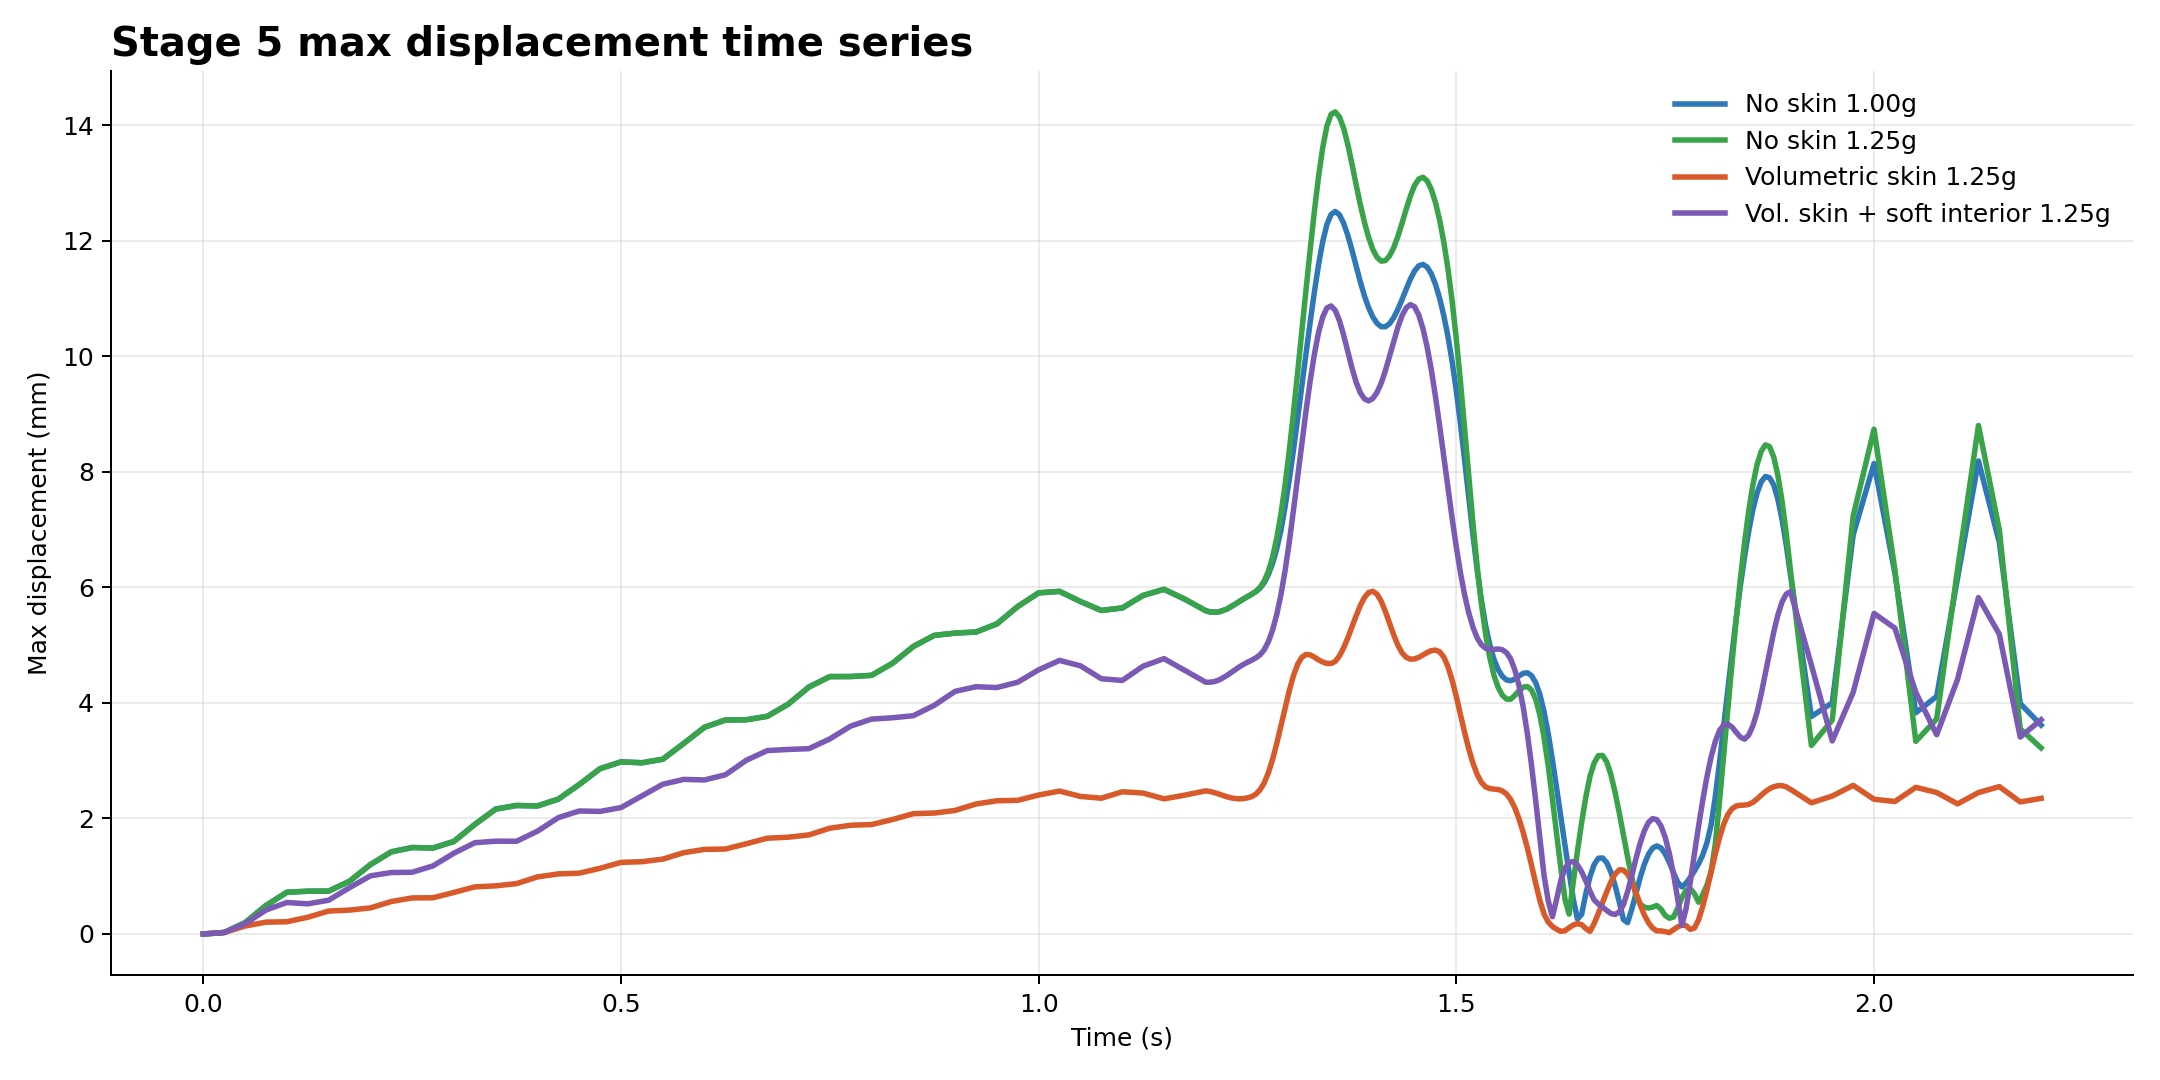
\includegraphics[width=0.95\linewidth]{Figures/stage5_manual_postprocess/stage5_manual_max_displacement_timeseries.png}
\caption{Manual Stage 5 maximum displacement time series. The volumetric skin cases follow the same broad dynamic pattern as the no-skin cases, but with lower amplitude. The soft-interior variant lies between the stiff volumetric-skin case and the no-skin cases.}
\label{fig:stage5_skin_scout_timeseries}
\end{figure}

The high maximum VM stress in the volumetric-skin cases occurred near the superior and inferior chestwall/support attachment region rather than as an isolated hotspot in the free breast volume. This supports interpretation as a local support/interface stress concentration. Therefore, the maximum VM value should be treated as a diagnostic hotspot metric, while average stress and displacement are more appropriate for global model comparison.

\begin{figure}[H]
\centering
\begin{subfigure}{0.32\linewidth}
\centering
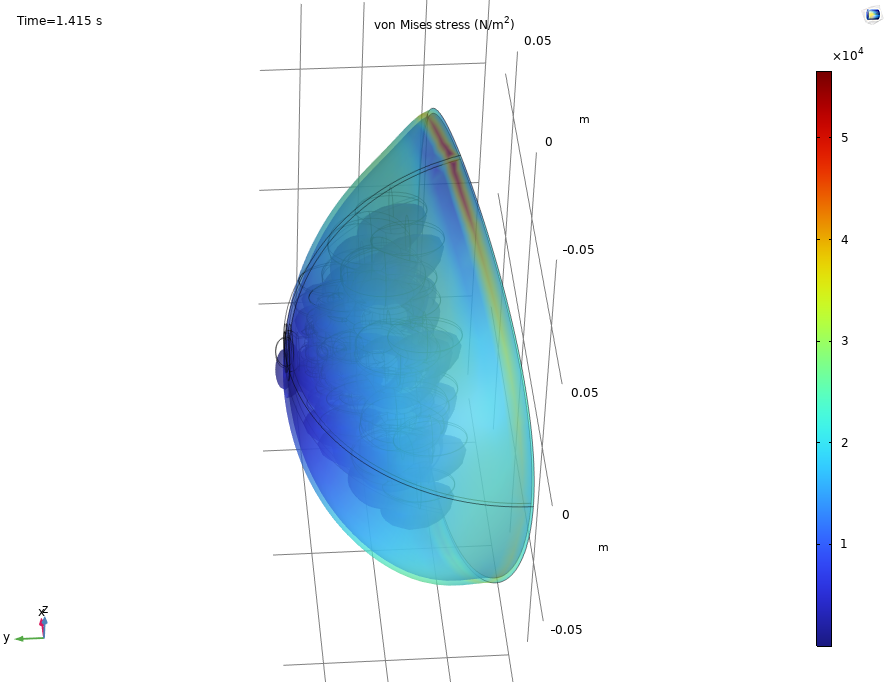
\includegraphics[width=\linewidth]{Figures/model_pictures/stage5_cooper/stage5_nocooper_125g_soft_interior_materials_vonMises_bovenaanzicht.png}
\caption{Superior view}
\end{subfigure}
\hfill
\begin{subfigure}{0.32\linewidth}
\centering
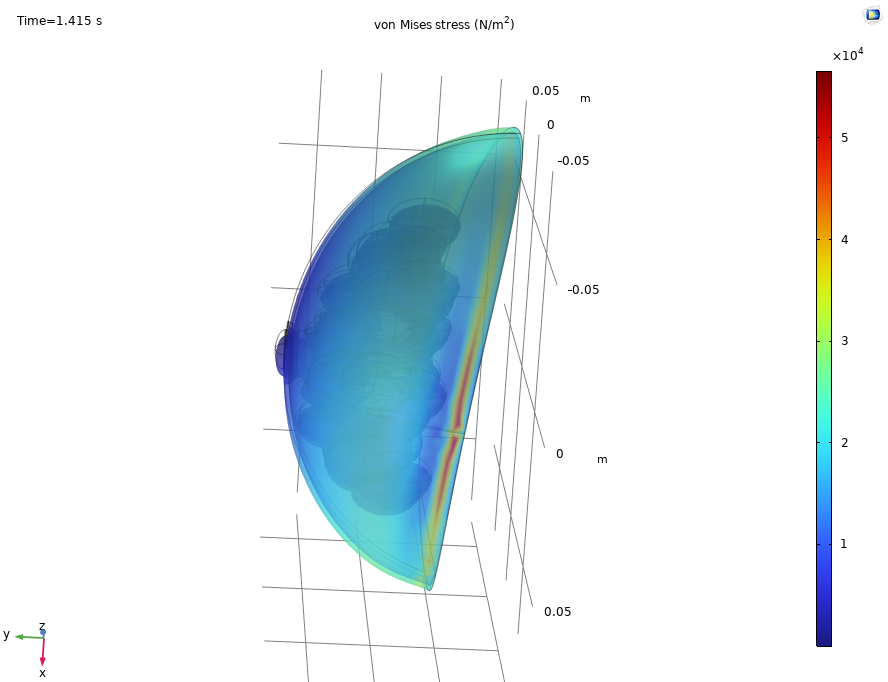
\includegraphics[width=\linewidth]{Figures/model_pictures/stage5_cooper/stage5_nocooper_125g_soft_interior_materials_vonMises_onderaanzicht.png}
\caption{Inferior view}
\end{subfigure}
\hfill
\begin{subfigure}{0.32\linewidth}
\centering
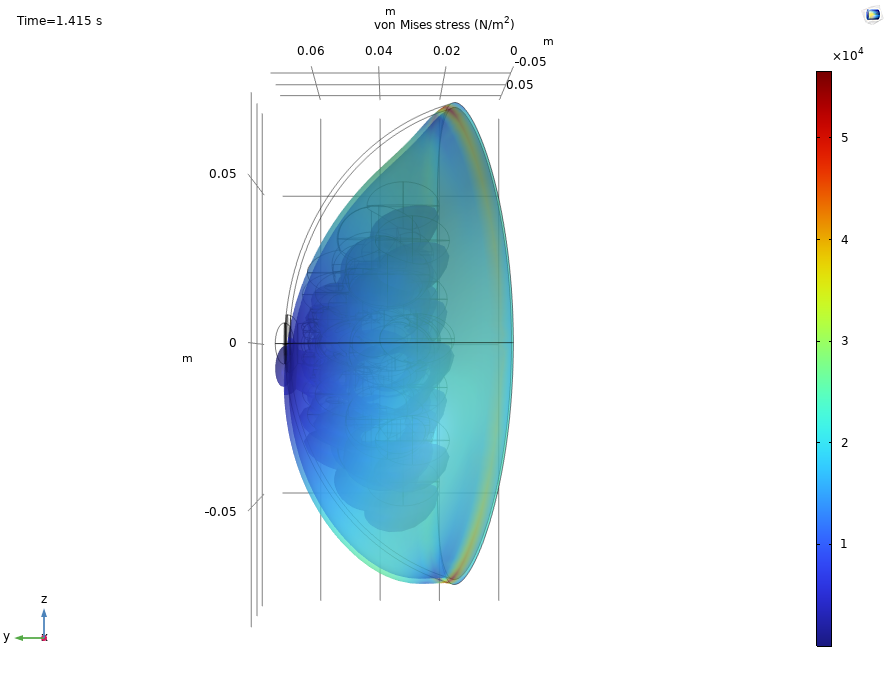
\includegraphics[width=\linewidth]{Figures/model_pictures/stage5_cooper/stage5_nocooper_125g_soft_interior_materials_vonMises_zijaanzicht.png}
\caption{Lateral view}
\end{subfigure}
\caption{Volumetric-skin soft-interior 1.25g VM stress distribution at the support/interface region. The peak stress is localized near the chestwall attachment rather than distributed through the free breast volume.}
\label{fig:stage5_volumetric_skin_stress_hotspots}
\end{figure}

\subsection{Stage 6: tumor/lesion build-screening route}

Stage 6 adds a first tumor/lesion sensitivity layer on top of the current anatomical route. The current implementation uses an analytic spherical tumor mask, not a separate tumor domain. The mask locally modifies density and Mooney--Rivlin coefficients and enables tumor-region volume, displacement, and stress metrics after a successful solve/postprocess step.

The Stage 6 screening set now contains a no-tumor control, a central size sweep, upper-outer, subareolar, posterior, and upper-outer surface-proximal candidates, plus mild/stiff material variants. The newest upper-outer candidates use small and medium spherical tumors in two visually checked positions: one closer to the inner breast surface and one more superior in the breast volume. These cases are intended to test whether tumor position and size produce measurable changes in global displacement, surface motion, nipple/landmark response, and local tumor-mask stress.

The current Stage 6 evidence should still be interpreted as build-screening and scout evaluation. The tumor sphere must be confirmed inside the breast union, and quantitative tumor conclusions should only be added after complete non-NaN tumor-mask metrics are available. The active fast-screening evaluation route is \texttt{analysis\_output/comsol\_pipeline/stage6\_fast\_tumor\_screening}; this folder should be used for early comparison plots, not as final clinical validation.

\subsection{Current best model interpretation}

The most defensible current model path is the Stage 2 xoffset055 chestwall baseline, the Stage 3 realistic glandular reference, a no-asymmetry control unless asymmetry is explicitly tested, and a no-Cooper control unless a stable Cooper support case is explicitly tested. Stage 6 should build from the same controlled reference. The current model is therefore strongest as a reproducible staged pipeline for sensitivity and diagnostic development, not yet as a patient-specific tumor detector.
